\section{Experiments on synthetic datasets\label{section:evaluation-experiments-on-synthetic-data}}

In addition to experiments on case-studies, QSM and ASM have been evaluated on synthetic datasets. The aim was to study their performance when the problem size, in terms of number of states of the target LTS, grows significantly beyond those of the case-studies. 
\begin{itemize}
\item This allow us to illustrate the expected performance of our algorithms on state machines whose size is more representative of real-world cases. 
\item It also provides performance profiles of our algorithms, for application contexts where the sizes of the target machines and/or of the learning samples are bigger than ours. These profiles are given in terms of accuracy, number of scenario questions and induction time reported for increasing learning sample sizes.
\end{itemize}

For reasons explained in Section~\ref{section:evaluation-objectives-and-approach}, however, we do not rely here on additional domain knowledge such as fluents, goals or models of legacy components.

Section~\ref{subsection:evaluation-synthetic-protocol} describes the methodology used to generate automata, learning and test samples. Section~\ref{subsection:evaluation-synthetic-qsm} then discusses the evaluation of QSM. Section~\ref{subsection:evaluation-synthetic-asm} discusses the one of ASM.

\subsection{Evaluation protocol\label{subsection:evaluation-synthetic-protocol}}

The procedure that has been used to evaluate ASM and QSM on synthetic data is inspired from the Abbadingo protocol \cite{Lang:1998}. Roughly, evaluating an induction algorithm consists in running it on learning samples of increasing size, in terms of their number of positive and negative strings. The accuracy of an induced model is then measured in terms of the number of strings of an independent test sample that the learned model correctly classifies.

Experiments here are made on random LTS of increasing sizes: $n$ = 20, 50, 100 and 200 states. Only alphabets of two symbols are considered, a feature inherited from Abbadingo\footnote{see Chapter \ref{chapter:stamina} for additional experiments on larger alphabets and a study of the influence of the alphabet size on induction algorithms.}. To match our application context, experiments here have been performed on LTS, not on the more general class of DFA (see Section \ref{section:background-lts-and-regular-languages}). In other words, all states of random automata are accepting states.

Inspired from Abbadingo, the randomly generated LTS are trimmed to remove unreachable states and minimized to obtain canonical target machines (see Section \ref{section:background-state-machines}). Moreover, only automata without terminating state are kept for the experiments. Such states typically capture deadlocks in multi-agent systems considered in our context and should therefore be avoided.

In order to build learning and test samples for a given target LTS, an initial set of $n^2$ different strings has been first synthesized. These strings are randomly generated without replacement using a uniform distribution over the collection of all binary strings of length $[0, p+5]$ where $p$ is the depth of the automaton. The depth of an automaton is defined as the length of the longest shortest path from the initial state to any other state. This bound is chosen so as to ensure that deepest states have a good change to be reached by at least one input string of a sample. This is a necessary condition for structural completeness of the sample (see Section \ref{section:inductive-background}), which was not guaranteed however.

Our procedure for generating samples is such that they contain positive and negative strings in roughly equal proportion.
 
A maximal sample size of $\frac{n^2}{2}$ strings was experimentally observed as offering the convergence for all tested algorithms (RPNI, Blue-fringe, QSM and ASM in different settings). The learning experiments have been conducted on increasing proportions of this nominal training sample, i.e. 3\%, 6\%, 12.5\%, 25\%, 50\% and 100\%.

Test samples of at most $\frac{n^2}{2}$ strings are used to measure the generalization accuracy of the learned model. The accuracy measure is precisely reported as the percentage of test strings correctly classified by the learned model.

Training and test samples are guaranteed not to overlap. Moreover, in the case of the QSM algorithm, test samples do not contain the additional strings that were submitted to the oracle during the interactive learning phase.

All experiments reported hereafter have been performed on at least 10 randomly generated LTS for each size and 5 randomly generated samples for each of them.

\subsection{Evaluation of QSM on synthetic datasets\label{subsection:evaluation-synthetic-qsm}}

This section reports evaluation results for the QSM algorithm. An automatic oracle has been implemented to answer the questions asked during its execution. This oracle correctly answers the membership queries since it has access to the target LTS in such controlled experiments.

\subsubsection*{Generalization accuracy}

Figure~\ref{image:evaluation-qsm-accuracy} reports, for several target sizes, the proportion of independent test samples correctly classified while increasing the learning sample size. Comparative performances are given for RPNI, Blue-fringe, QSM-rpni (QSM with the RPNI merging order) and QSM-fringe (QSM with the Blue-fringe strategy).

\begin{figure}[t]
\centering
\scalebox{.25}{
  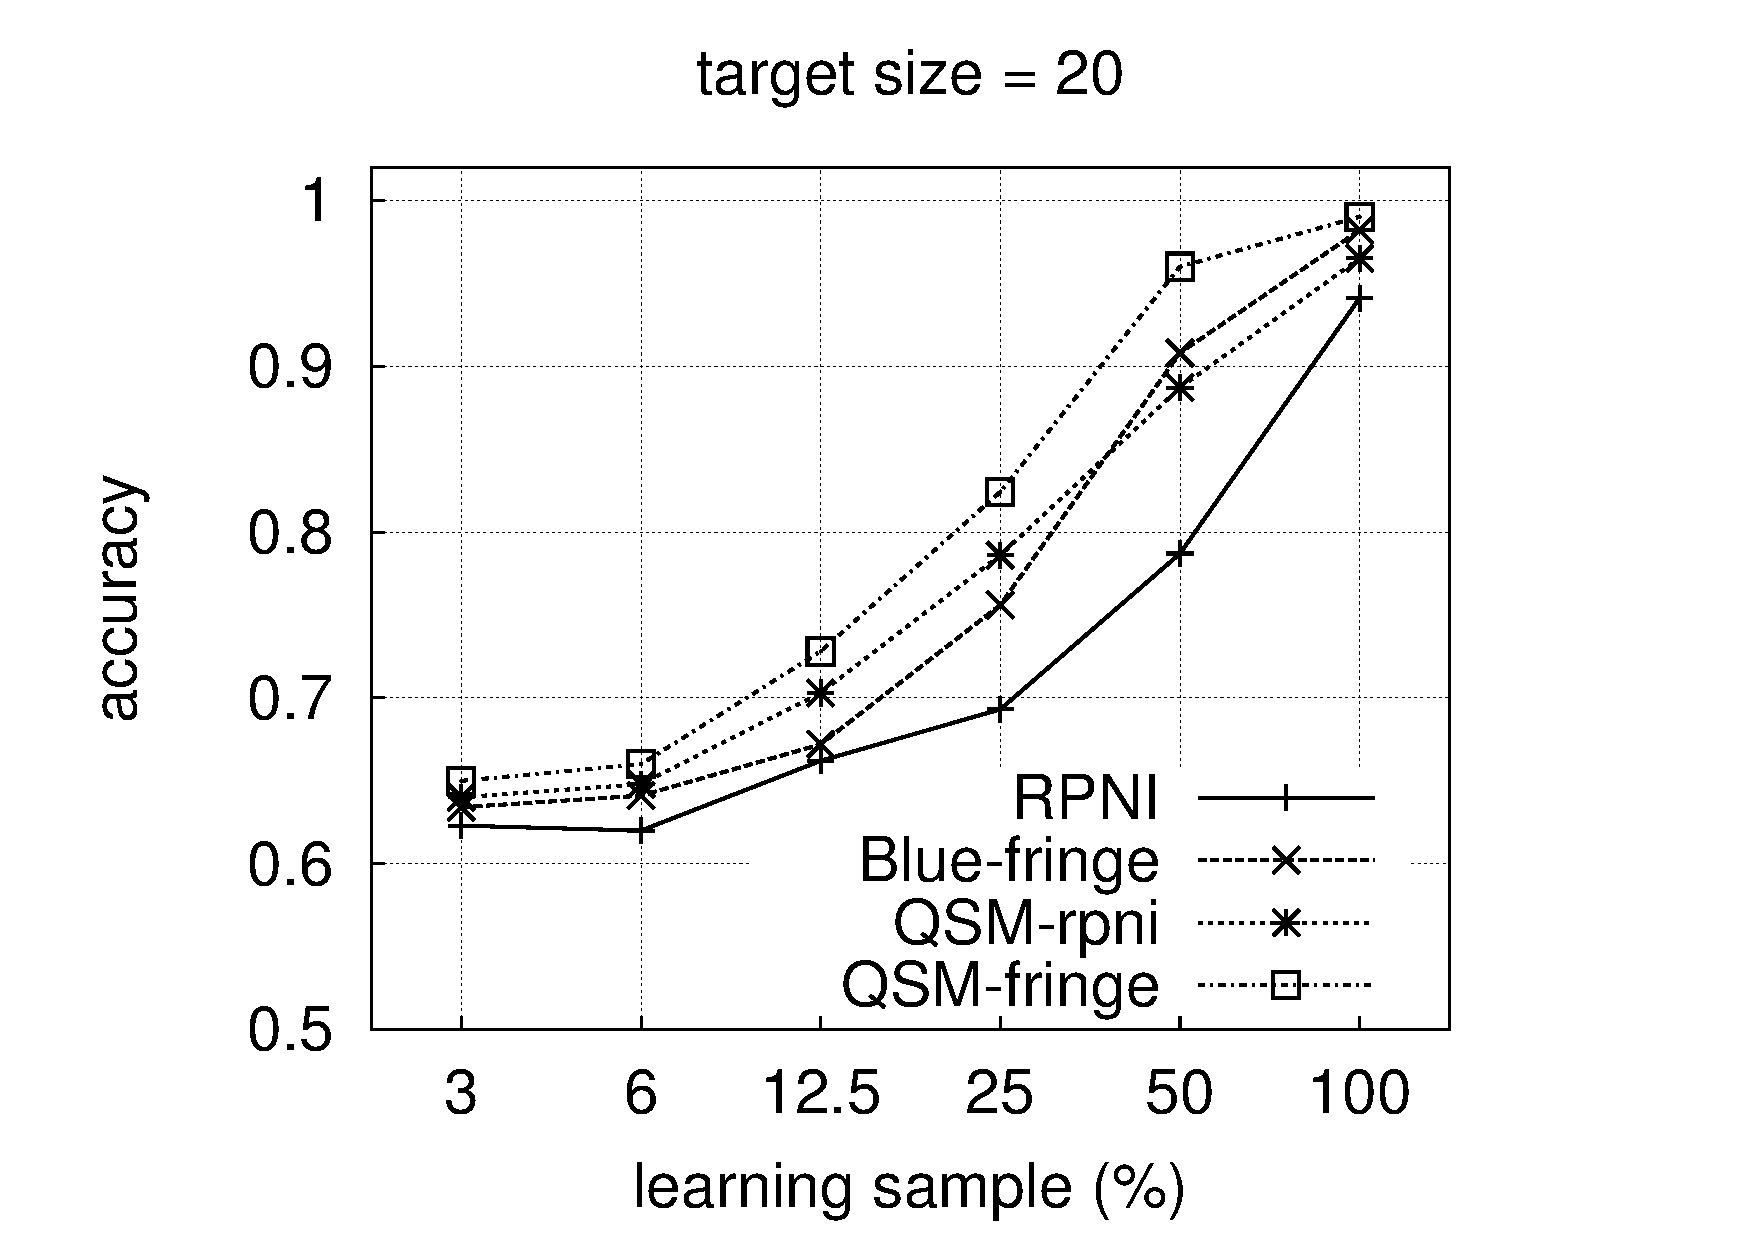
\includegraphics[trim=0mm  21mm 45mm 0mm, clip, page=1]{src/5-evaluation/images/accuracy}
  \includegraphics[trim=30mm 21mm 35mm 0mm, clip, page=2]{src/5-evaluation/images/accuracy}
}\vspace{0.35cm}
\scalebox{.25}{
  \includegraphics[trim=0mm  0mm 45mm 0mm, clip, page=3]{src/5-evaluation/images/accuracy}
  \includegraphics[trim=30mm 0mm 35mm 0mm, clip, page=4]{src/5-evaluation/images/accuracy}
}
\caption{Classification accuracy of QSM\label{image:evaluation-qsm-accuracy}.}
\end{figure}

Results from Section \ref{subsection:evaluation-bluefringe-on-casestudies} on case-studies are confirmed here since Blue-fringe (resp. QSM-fringe) outperforms RPNI (resp. QSM-rpni) for sparse training samples. Moreover, significant improvements of the generalization accuracy is observed thanks to the interactive feature:
\begin{itemize}
\item The QSM algorithm outperforms the original RPNI and Blue-fringe systematically.
\item Interestingly, QSM-rpni also overcomes the original Blue-fringe algorithm. In terms of model accuracy and for a fixed learning sample size, the interactive feature of QSM is at least as powerful as the evidence-driven search heuristic of Blue-fringe.
\end{itemize}

Observe that the learning sample sizes are well chosen to illustrate the convergence of this family of induction algorithms:
\begin{itemize}
\item For a given target size, the curves show the different induction phases. When the sample is sparse, 3\% or 6\% for example, poor accuracy results are first observed. The accuracy grows while the learning sample becomes larger; it does so rapidely until an accuracy of about 0.95 is reached. Beyond this point, the accuracy continues to grow with the learning sample size but much slowly. 
\item The relative performances described above do not depend much on the target size. However, the curves seem successively shifted left when the target size grows. This can be explained by the fact that a quadratic learning sample with respect to the size of the target LTS tend to be richer for large LTS than for the small ones. 
\end{itemize}

\subsubsection*{Number of queries\label{subsection:evaluation-synthetic-queries-on-qsm}}

An important aspect of QSM is the number of queries submitted to the oracle. When the oracle is an end-user, this factor indeed drives the usability of the approach in practice. 

Figure~\ref{image:evaluation-qsm-number-of-questions} presents the number of generated queries depending on the learning sample size, for several target sizes. Results are given for QSM-rpni and QSM-fringe. In each case, the number of generated strings which are classified by the oracle either as positive or negative are reported separately.

\begin{itemize}
\item The number of strings classified as positive tends to increase initially with the learning sample size before staying roughly constant when the learning process has nearly converged. The additional information required to guarantee correct identification mostly depends on the negative strings.
\item QSM-fringe tends to generate fewer strings classified as negative by the oracle than QSM-rpni. In both cases, however, the number of rejected queries decreases with the learning sample size. As a comparison of Fig.~\ref{image:evaluation-qsm-number-of-questions} and Fig~\ref{image:evaluation-qsm-accuracy} shows, it even reaches zero when the algorithm has converged toward the exact model.
\end{itemize}

\begin{figure}
\centering
\scalebox{.25}{
  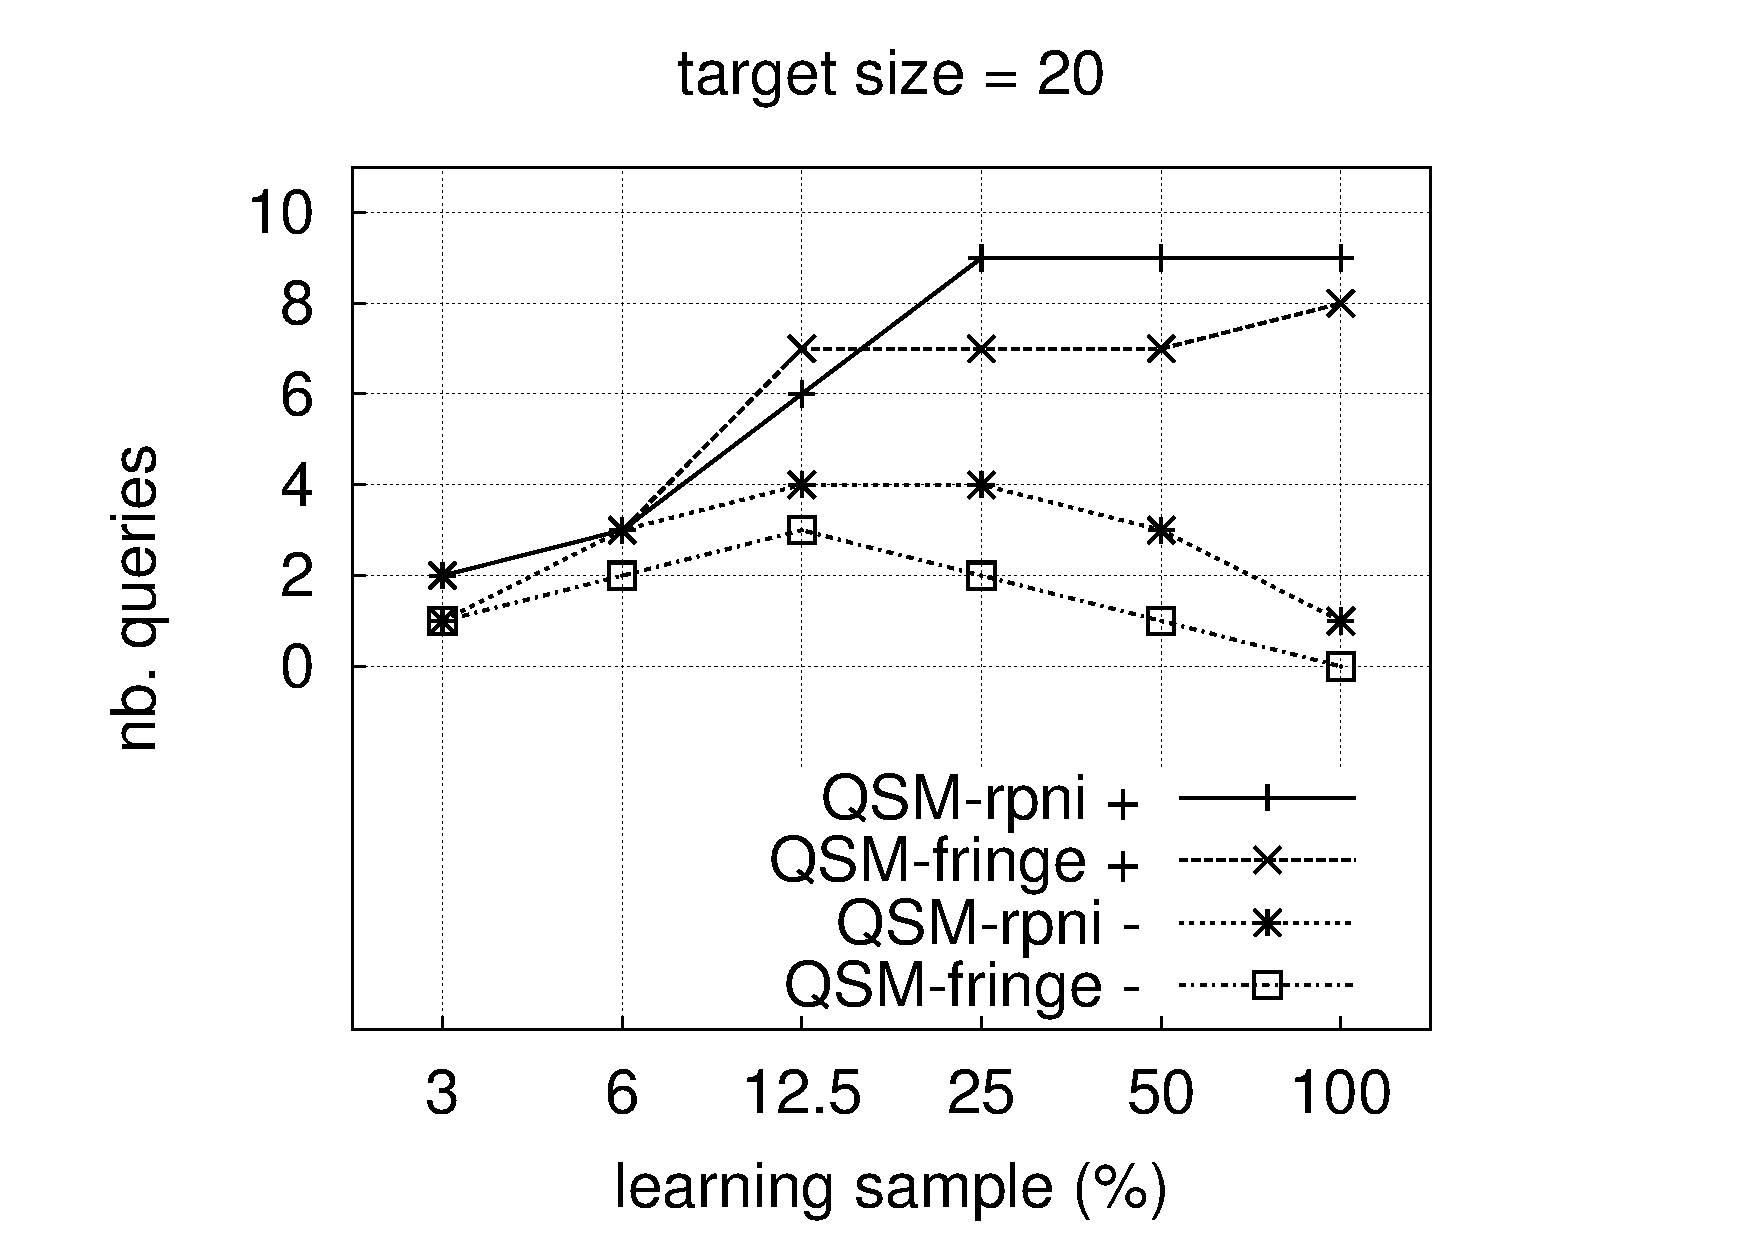
\includegraphics[trim=0mm  21mm 45mm 0mm, clip, page=1]{src/5-evaluation/images/queries}
  \includegraphics[trim=30mm 21mm 35mm 0mm, clip, page=2]{src/5-evaluation/images/queries}
}\vspace{0.35cm}
\scalebox{.25}{
  \includegraphics[trim=0mm  0mm 45mm 0mm, clip, page=3]{src/5-evaluation/images/queries}
  \includegraphics[trim=30mm 0mm 35mm 0mm, clip, page=4]{src/5-evaluation/images/queries}
}
\caption{Number of queries generated by QSM\label{image:evaluation-qsm-number-of-questions}.}
\end{figure}

\subsubsection*{Induction time\label{cpu:time}}

Figure~\ref{image:evaluation-qsm-time} reports the induction time while varying learning sample size and target size. All tests were executed with Java 5.0 on a Pentium-IV 3 GHz computer with 1Gb of RAM. 

The RPNI, Blue-fringe and QSM algorithms go through different phases according to the amount of available data:
\begin{itemize} 
\item Initially, the CPU time tends to increase with the learning sample size. In this first phase, the learning time follows the increase of the sample size. 
\item When the learning sample becomes richer, better generalizations can be obtained by merging states in a more sound way. A comparison between curves in Fig.~\ref{image:evaluation-qsm-accuracy} and in Fig.~\ref{image:evaluation-qsm-time} shows that the classification rates of new data increases while the learning time reaches its maximum. 
\item The last phase is observed when the algorithm rapidly converges to a good model. Classification accuracy tends to 100\% and the CPU time is decreased because the right merging operations are performed directly. 
\end{itemize}

\begin{figure}[t]
\centering
\scalebox{.25}{
  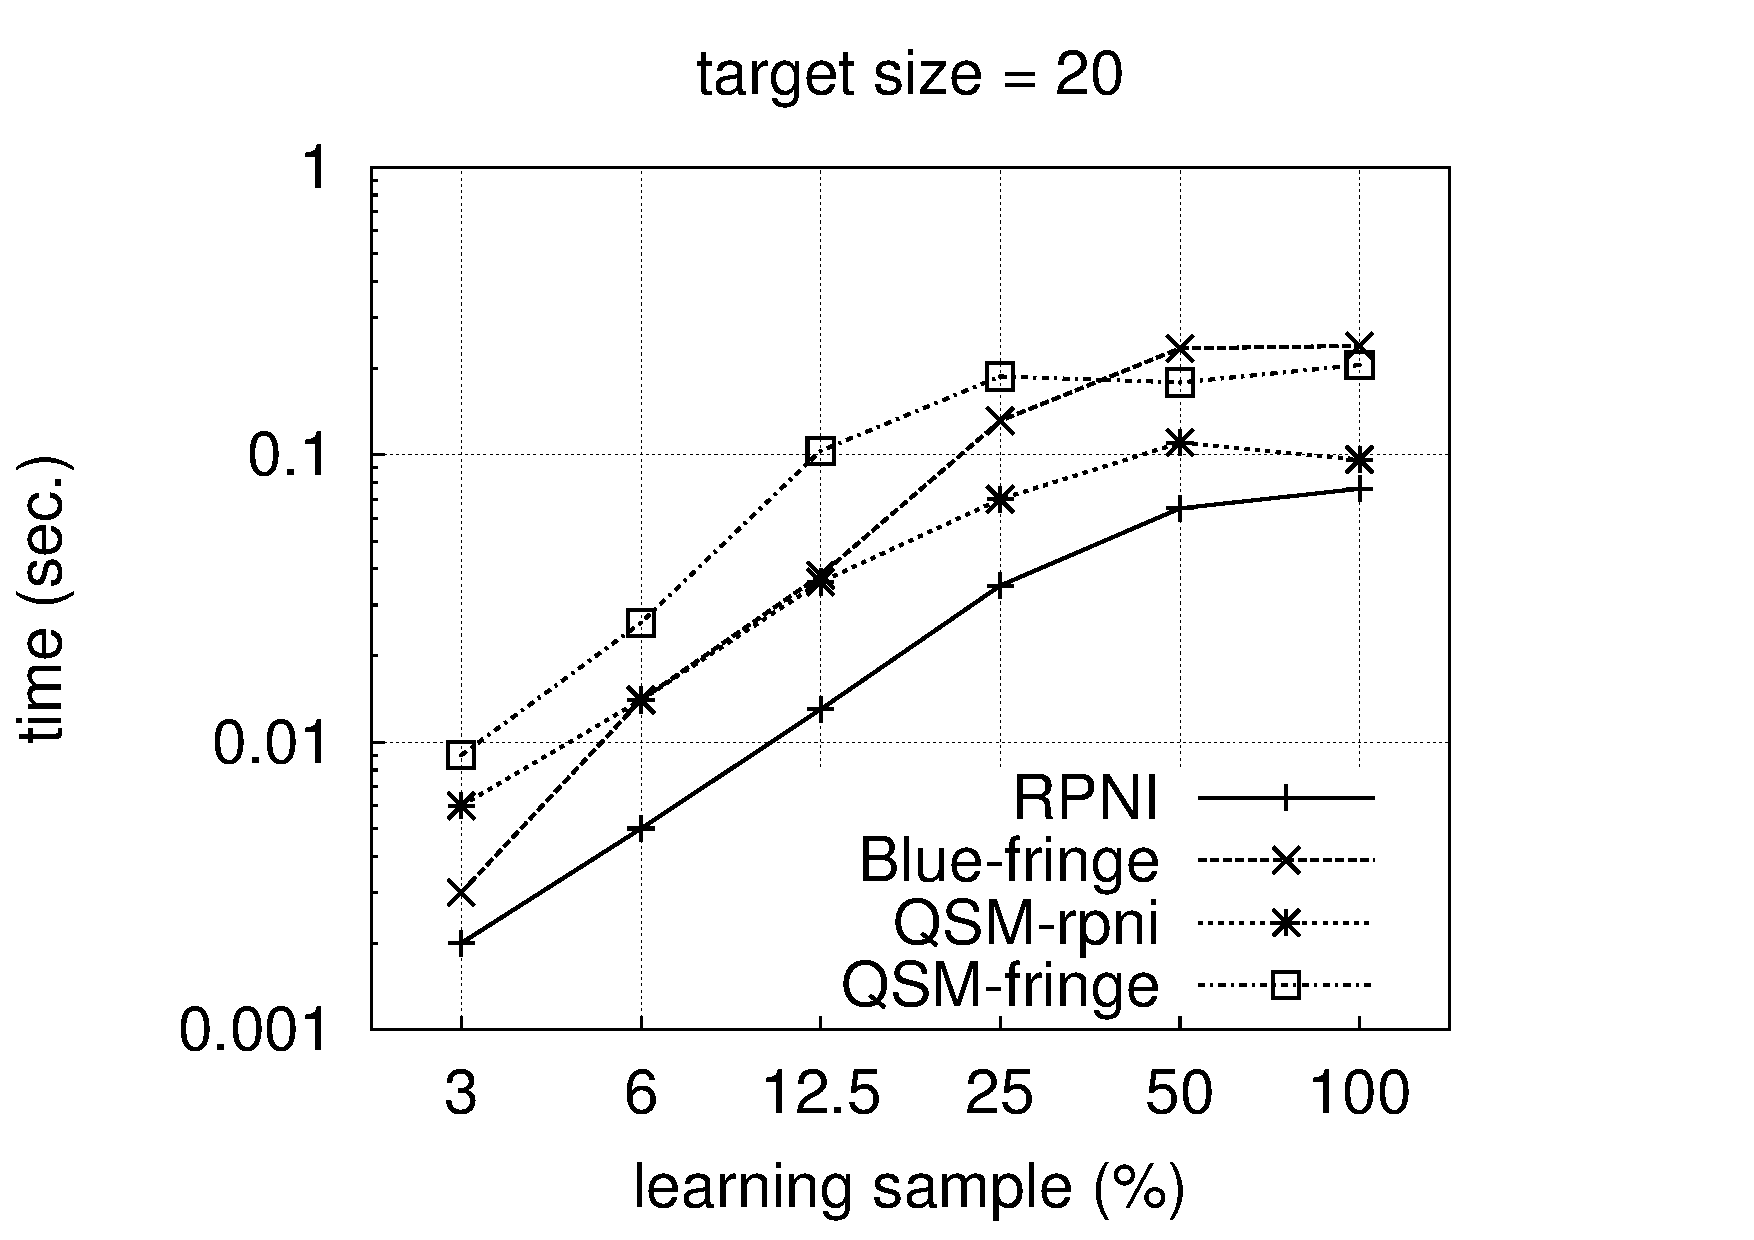
\includegraphics[trim=0mm  21mm 45mm 0mm, clip, page=1]{src/5-evaluation/images/time}
  \includegraphics[trim=30mm 21mm 35mm 0mm, clip, page=2]{src/5-evaluation/images/time}
}\vspace{0.35cm}
\scalebox{.25}{
  \includegraphics[trim=0mm  0mm 45mm 0mm, clip, page=3]{src/5-evaluation/images/time}
  \includegraphics[trim=30mm 0mm 35mm 0mm, clip, page=4]{src/5-evaluation/images/time}
}
\caption{Induction time with QSM\label{image:evaluation-qsm-time}.}
\end{figure}

Known tendencies of induction algorithms of the RPNI family are confirmed in our experiments (see, e.g., \cite{Lang:1998}). However, the curves of QSM are shifted left with respect to the learning sample size. As already observed in Fig.~\ref{image:evaluation-qsm-accuracy}, convergence is indeed faster for the QSM algorithm in that it occurs on sparser samples than with RPNI or Blue-fringe. The relative time performance of the QSM algorithm with respect to them actually depends on two contradictory effects:
\begin{itemize}
\item On the one hand, whenever a string is classified as negative by the oracle, QSM is called recursively on an extended sample. Each new call increases the CPU time as it could be considered as a new run of the RPNI or Blue-fringe algorithm. This run can however be interrupted and replaced by another one if a new negative example is included after an additional query.
\item On the other hand, due to its faster convergence, QSM can obtain better results with fewer data originally provided. 
\end{itemize}
 
The CPU times should thus be compared while considering the relative classification results of the various approaches. For instance, when the target size is 200 and 3\% of the full training sample is used, QSM-fringe runs an order of magnitude slower than Blue-fringe. However, the classification accuracy of QSM-fringe is 95\% while it is 67\% for Blue-fringe for the same amount of data. When the training size increases, QSM-fringe actually becomes slightly faster than Blue-fringe because it has already nearly converged to the optimal solution.

\subsection{Evaluation of ASM on synthetic datasets\label{subsection:evaluation-synthetic-asm}}

The evaluation of ASM on synthetic data is very similar to the one conducted on case-studies in Section \ref{subsection:evaluation-casestudies-asm}. The objective is to quantify the gain of generalization accuracy that can be expected when the proportion of domain-specific control information, such as a hMSC, is increased as input. 

The experimentation protocol that we used to achieve this objective is a slight adaptation of the one discussed in Section \ref{subsection:evaluation-synthetic-protocol}:
\begin{itemize}
\item Experiments here are made on randomly generated target LTS with 32 and 64 states. Following Abbadingo, alphabets still have two symbols only (we further discuss this limitation in Chapter~\ref{chapter:stamina}).
\item Learning and test samples are randomly generated as before. RPNI and Blue-fringe are both evaluated on these samples to provide a reference for the comparisons with ASM.  
\item In order to provide its input to ASM, a specific procedure simulates the control information given by a hMSC:
\begin{itemize}
\item For a given learning sample, an augmented PTA is first built. As in Section \ref{subsection:evaluation-casestudies-asm}, an early state merging phase then occurs. The idea is to merge specific state pairs of the PTA that are known to correspond to the same state in the target LTS.
\item Unique labels are associated to randomly chosen states of the target LTS. Increasing proportions of the number of states labeled in this way have been used: 5\%, 10\%, 20\% and 100\%. The PTA and the target LTS are then jointly visited and state labels are reported as decorations of the PTA states. 
\item States of the PTA sharing the same label are merged early. This effectively simulates the availability of control information through a hMSC, by introducing loops in the input scenarios. The automaton resulting from this step is then used as input of ASM, that further generalizes it by merging additional state pairs under the control of the negative strings.
\end{itemize}
\end{itemize}
 
Figure~\ref{image:evaluation-asm-accuracy} reports the proportion of independent test samples correctly classified while increasing the learning sample. Curves in this plots correspond to executions of RPNI, Blue-fringe and ASM with different labeling proportions. Each point in these plots is the average value computed over 200 independent runs. 

\begin{figure}
\begin{center}
\scalebox{.28}{\includegraphics*{src/5-evaluation/images/asm-accuracy.jpg}}
\caption{Classification accuracy for ASM\label{image:evaluation-asm-accuracy}.}
\end{center}
\end{figure}

ASM overcomes RPNI on all executions, which is actually expected. Remember from Section~\ref{subsection:automaton-state-merging} that ASM reduces to RPNI in the special case where its input is a PTA, that is, when no early state merging occurs in our experiment. By construction of our experiments, the early state merging performed are sound. Therefore, they could not hurt the obtained generalization accuracy; hence, ASM can only obtain the same or a better accuracy score than RPNI.

Observe, however, that 5\% of labeling information is comparable, from the point of view of the generalization accuracy, to the use of the Blue-fringe heuristic for selecting state pairs to be merged. Beyond this proportion, the accuracy continues to increase. Interestingly, the accuracy gain is already visible when the sample is sparse.

Note that the identification of the target does not reduce to a trivial problem even with 100\% of labeling information. As discussed in Section \ref{section:inductive-from-hMSC}, control information is complementary but does substitute to the negative knowledge provided by negative scenarios, fluent and goals. In particular, it does not prevent over-generalization occuring from incompatible state pairs being merged. 
